\documentclass{standalone}
\usepackage{tikz}
\usetikzlibrary{calc,arrows.meta,decorations.markings,math,patterns}
%\ifpdftex\usepackage[scaled=1]{helvet}\fi
\ifxetex\usepackage{fontspec}\setsansfont{TeX Gyre Heros}\fi
\begin{document}
\begingroup
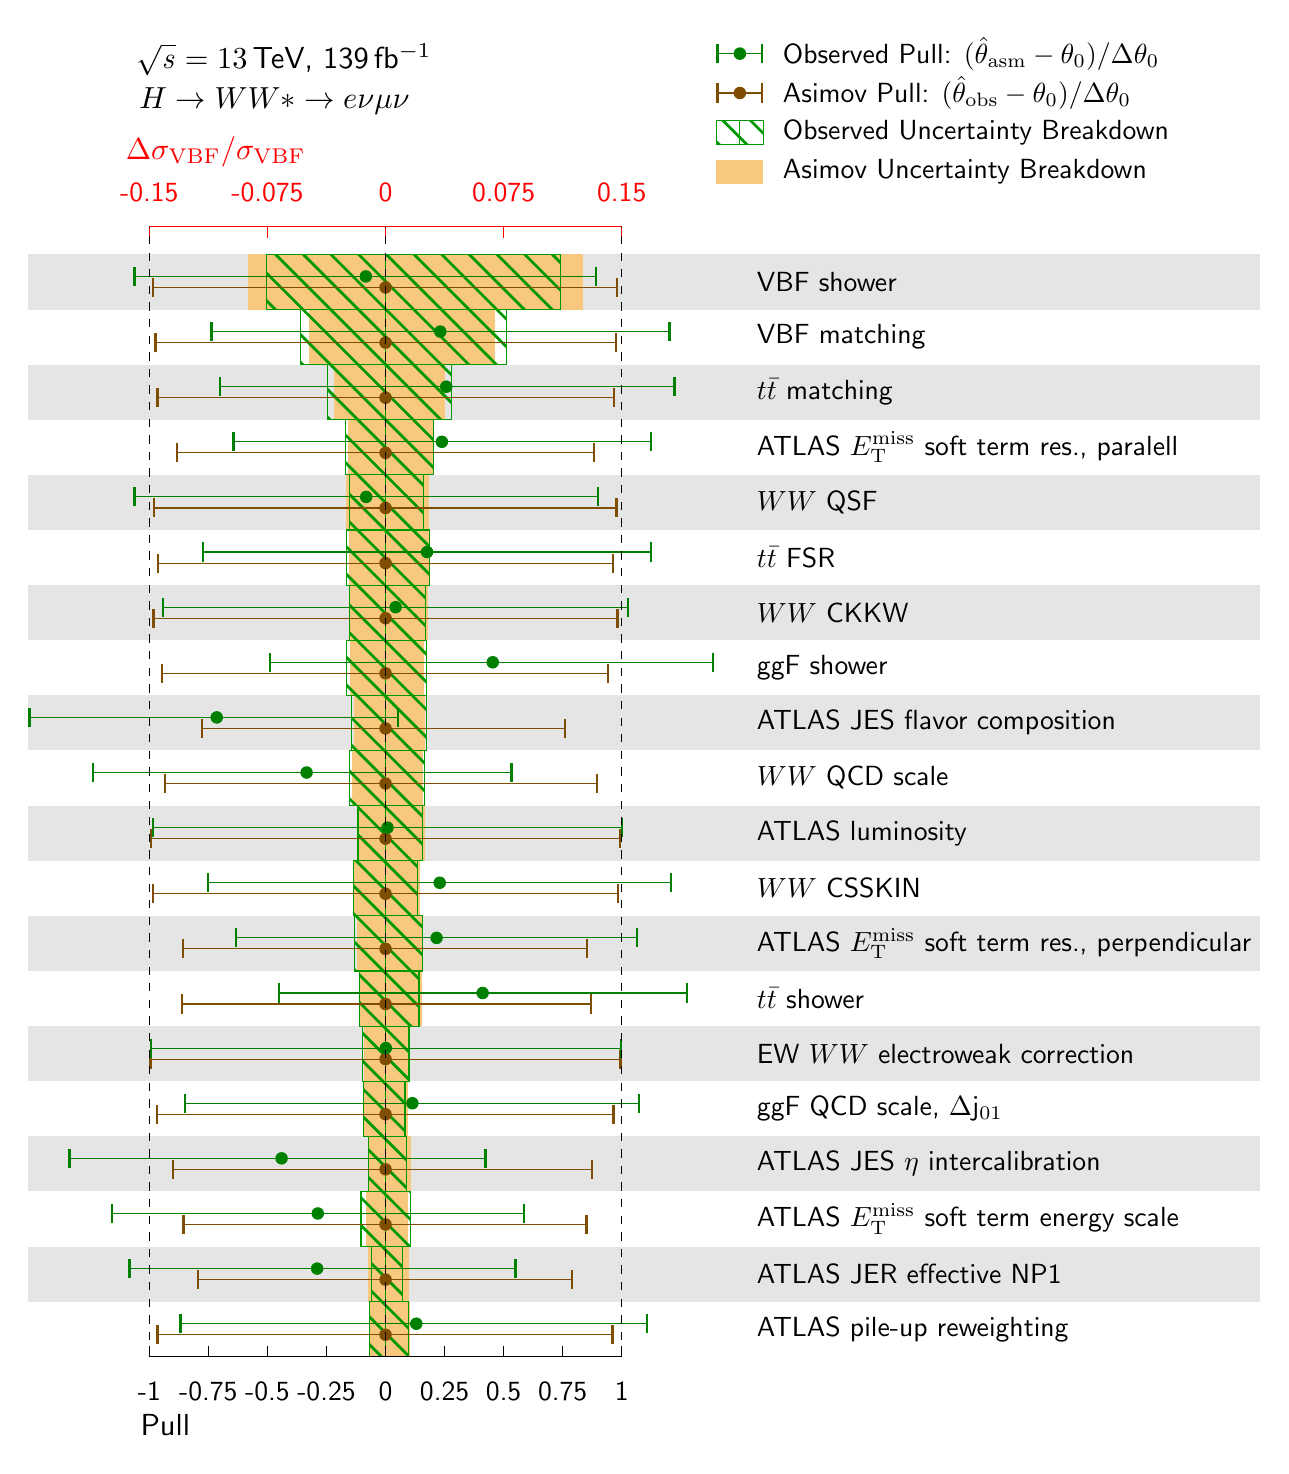
\begin{tikzpicture}[x=3cm,y=.7cm,%
  axlbl/.style={scale=1,anchor=center},%
  pull/.style={{|[scale=1.5, line width=0.3mm]}-{|[scale=1.5, line width=0.3mm]}},%scale is error vertical bar size
  dot/.style={circle,fill,inner sep=1pt,scale=1.6},
  every node/.append style={line width=2mm,font=\sffamily}
]

  % defining the new dimensions and parameters
\newlength{\hatchspread}
\newlength{\hatchthickness}
\newlength{\hatchshift}
\newcommand{\hatchcolor}{}
% declaring the keys in tikz
\tikzset{hatchspread/.code={\setlength{\hatchspread}{#1}},
         hatchthickness/.code={\setlength{\hatchthickness}{#1}},
         hatchshift/.code={\setlength{\hatchshift}{#1}},% must be >= 0
         hatchcolor/.code={\renewcommand{\hatchcolor}{#1}}}
% setting the default values
\tikzset{hatchspread=1pt,
         hatchthickness=1pt,
         hatchshift=0pt,% must be >= 0
         hatchcolor=black}
% declaring the pattern
\pgfdeclarepatternformonly[\hatchspread,\hatchthickness,\hatchshift,\hatchcolor]% variables
   {custom north west lines}% name
   {\pgfqpoint{\dimexpr-2\hatchthickness}{\dimexpr-2\hatchthickness}}% lower left corner
   {\pgfqpoint{\dimexpr\hatchspread+2\hatchthickness}{\dimexpr\hatchspread+2\hatchthickness}}% upper right corner
   {\pgfqpoint{\dimexpr\hatchspread}{\dimexpr\hatchspread}}% tile size
   {% shape description
    \pgfsetlinewidth{\hatchthickness}
    \pgfpathmoveto{\pgfqpoint{0pt}{\dimexpr\hatchspread+\hatchshift}}
    \pgfpathlineto{\pgfqpoint{\dimexpr\hatchspread+0.15pt+\hatchshift}{-0.15pt}}
    \ifdim \hatchshift > 0pt
      \pgfpathmoveto{\pgfqpoint{0pt}{\hatchshift}}
      \pgfpathlineto{\pgfqpoint{\dimexpr0.15pt+\hatchshift}{-0.15pt}}
    \fi
    \pgfsetstrokecolor{\hatchcolor}
    \pgfusepath{stroke}
   }
  
\definecolor{colOverlay.Ranking.BREAKDOWNS.observedTwoPos}{rgb}{0.972549,0.784314,0.498039}
\definecolor{colOverlay.Ranking.BREAKDOWNS.observedTwoNeg}{rgb}{0.972549,0.784314,0.498039}
\definecolor{colOverlay.Ranking.BREAKDOWNS.observedTwoHatchPos}{rgb}{0.972549,0.784314,0.498039}
\definecolor{colOverlay.Ranking.BREAKDOWNS.observedTwoHatchNeg}{rgb}{0.972549,0.784314,0.498039}
\tikzset{Overlay.Ranking.BREAKDOWNS.observedTwoPos/.style={draw=none,fill=colOverlay.Ranking.BREAKDOWNS.observedTwoPos,text opacity = 1.0, fill opacity=1,}}
\tikzset{Overlay.Ranking.BREAKDOWNS.observedTwoNeg/.style={draw=none,fill=colOverlay.Ranking.BREAKDOWNS.observedTwoNeg,text opacity = 1.0, fill opacity=1,}}
\definecolor{colOverlay.Ranking.BREAKDOWNS.observedPos}{rgb}{0.000000,0.600000,0.000000}
\definecolor{colOverlay.Ranking.BREAKDOWNS.observedNeg}{rgb}{0.000000,0.600000,0.000000}
\definecolor{colOverlay.Ranking.BREAKDOWNS.observedHatchPos}{rgb}{0.000000,0.600000,0.000000}
\definecolor{colOverlay.Ranking.BREAKDOWNS.observedHatchNeg}{rgb}{0.000000,0.600000,0.000000}
\tikzset{Overlay.Ranking.BREAKDOWNS.observedPos/.style={draw=colOverlay.Ranking.BREAKDOWNS.observedPos,pattern=custom north west lines, hatchcolor=colOverlay.Ranking.BREAKDOWNS.observedHatchPos,hatchspread=10pt,}}
\tikzset{Overlay.Ranking.BREAKDOWNS.observedNeg/.style={draw=colOverlay.Ranking.BREAKDOWNS.observedNeg,pattern=custom north west lines, hatchcolor=colOverlay.Ranking.BREAKDOWNS.observedHatchNeg,hatchspread=10pt,}}
\definecolor{colEffectAxes}{rgb}{1.000000,0.000000,0.000000}
%\definecolor{colOverlay.Pulls.PULLS.observedTwo}{rgb}{0.968627,0.611765,0.066667}
\definecolor{colOverlay.Pulls.PULLS.observedTwo}{rgb}{0.501961,0.305882,0.011765}
\tikzset{Overlay.Pulls.PULLS.observedTwo/.style={pull,color=colOverlay.Pulls.PULLS.observedTwo}}
%\definecolor{colOverlay.Pulls.PULLS.observed}{rgb}{0.000000,0.600000,0.000000}
\definecolor{colOverlay.Pulls.PULLS.observed}{rgb}{0.000000,0.500000,0.000000}
\tikzset{Overlay.Pulls.PULLS.observed/.style={pull,color=colOverlay.Pulls.PULLS.observed}}
\definecolor{colPullAxes}{rgb}{0.000000,0.000000,0.000000}
\definecolor{colHighlighting}{rgb}{0.900000,0.900000,0.900000}
\begin{scope}[name=legend,shift={(1.5,1)},x=0.3cm,y=.5cm]\draw[Overlay.Ranking.BREAKDOWNS.observedTwoNeg](-1,-0.3) rectangle (0,0.3);
\draw[Overlay.Ranking.BREAKDOWNS.observedTwoPos](0,-0.3) rectangle (1,0.3);
\node[anchor=west] at(1.1,0){Asimov Uncertainty Breakdown};
\draw[Overlay.Ranking.BREAKDOWNS.observedNeg](-1,0.7) rectangle (0,1.3);
\draw[Overlay.Ranking.BREAKDOWNS.observedPos](0,0.7) rectangle (1,1.3);
\node[anchor=west] at(1.1,1){Observed Uncertainty Breakdown};
\draw[Overlay.Pulls.PULLS.observedTwo](-1,2) -- (1,2);\node[dot,colOverlay.Pulls.PULLS.observedTwo] at (0,2) {};
\node[anchor=west] at(1.1,2){Asimov Pull: $(\hat{\theta}_{\mathrm{obs}} - \theta_0) / \Delta \theta_0$};
\draw[Overlay.Pulls.PULLS.observed](-1,3) -- (1,3);\node[dot,colOverlay.Pulls.PULLS.observed] at (0,3) {};
\node[anchor=west] at(1.1,3){Observed Pull: $(\hat{\theta}_{\mathrm{asm}} - \theta_0) / \Delta \theta_0$};
\end{scope}\pgfdeclarelayer{background}\pgfsetlayers{background,main}
\node[scale=1,anchor=west,rotate=0] at (1.5,-1) {VBF shower};
\node[scale=1,anchor=west,rotate=0] at (1.5,-2) {VBF matching};
\node[scale=1,anchor=west,rotate=0] at (1.5,-3) {$t\bar{t}$ matching};
\node[scale=1,anchor=west,rotate=0] at (1.5,-4) {ATLAS $E_{\rm T}^{\mathrm{miss}}$ soft term res., paralell};
\node[scale=1,anchor=west,rotate=0] at (1.5,-5) {$WW$ QSF};
\node[scale=1,anchor=west,rotate=0] at (1.5,-6) {$t\bar{t}$ FSR};
\node[scale=1,anchor=west,rotate=0] at (1.5,-7) {$WW$ CKKW};
\node[scale=1,anchor=west,rotate=0] at (1.5,-8) {ggF shower};
\node[scale=1,anchor=west,rotate=0] at (1.5,-9) {ATLAS JES flavor composition};
\node[scale=1,anchor=west,rotate=0] at (1.5,-10) {$WW$ QCD scale};
\node[scale=1,anchor=west,rotate=0] at (1.5,-11) {ATLAS luminosity};
\node[scale=1,anchor=west,rotate=0] at (1.5,-12) {$WW$ CSSKIN};
\node[scale=1,anchor=west,rotate=0] at (1.5,-13) {ATLAS $E_{\rm T}^{\mathrm{miss}}$ soft term res., perpendicular};
\node[scale=1,anchor=west,rotate=0] at (1.5,-14) {$t\bar{t}$ shower};
\node[scale=1,anchor=west,rotate=0] at (1.5,-15) {EW $WW$ electroweak correction};
\node[scale=1,anchor=west,rotate=0] at (1.5,-16) {ggF QCD scale, $\Delta $j$_{01}$};
\node[scale=1,anchor=west,rotate=0] at (1.5,-17) {ATLAS JES $\eta$ intercalibration};
\node[scale=1,anchor=west,rotate=0] at (1.5,-18) {ATLAS $E_{\rm T}^{\mathrm{miss}}$ soft term energy scale};
\node[scale=1,anchor=west,rotate=0] at (1.5,-19) {ATLAS JER effective NP1};
\node[scale=1,anchor=west,rotate=0] at (1.5,-20) {ATLAS pile-up reweighting};
\begin{scope}[name=ranking,colEffectAxes,xscale=6.66667]
    \draw[Overlay.Ranking.BREAKDOWNS.observedTwoNeg](-0.0876475,-1.5) rectangle (0,-0.5);
    \draw[Overlay.Ranking.BREAKDOWNS.observedTwoPos](0,-1.5) rectangle (0.125595,-0.5);
    \draw[Overlay.Ranking.BREAKDOWNS.observedTwoNeg](-0.0485637,-2.5) rectangle (0,-1.5);
    \draw[Overlay.Ranking.BREAKDOWNS.observedTwoPos](0,-2.5) rectangle (0.0697954,-1.5);
    \draw[Overlay.Ranking.BREAKDOWNS.observedTwoNeg](-0.0327105,-3.5) rectangle (0,-2.5);
    \draw[Overlay.Ranking.BREAKDOWNS.observedTwoPos](0,-3.5) rectangle (0.0377809,-2.5);
    \draw[Overlay.Ranking.BREAKDOWNS.observedTwoNeg](-0.0238198,-4.5) rectangle (0,-3.5);
    \draw[Overlay.Ranking.BREAKDOWNS.observedTwoPos](0,-4.5) rectangle (0.0299959,-3.5);
    \draw[Overlay.Ranking.BREAKDOWNS.observedTwoNeg](-0.0248989,-5.5) rectangle (0,-4.5);
    \draw[Overlay.Ranking.BREAKDOWNS.observedTwoPos](0,-5.5) rectangle (0.0274559,-4.5);
    \draw[Overlay.Ranking.BREAKDOWNS.observedTwoNeg](-0.0233459,-6.5) rectangle (0,-5.5);
    \draw[Overlay.Ranking.BREAKDOWNS.observedTwoPos](0,-6.5) rectangle (0.0274569,-5.5);
    \draw[Overlay.Ranking.BREAKDOWNS.observedTwoNeg](-0.0230997,-7.5) rectangle (0,-6.5);
    \draw[Overlay.Ranking.BREAKDOWNS.observedTwoPos](0,-7.5) rectangle (0.026786,-6.5);
    \draw[Overlay.Ranking.BREAKDOWNS.observedTwoNeg](-0.0224591,-8.5) rectangle (0,-7.5);
    \draw[Overlay.Ranking.BREAKDOWNS.observedTwoPos](0,-8.5) rectangle (0.0242266,-7.5);
    \draw[Overlay.Ranking.BREAKDOWNS.observedTwoNeg](-0.0200373,-9.5) rectangle (0,-8.5);
    \draw[Overlay.Ranking.BREAKDOWNS.observedTwoPos](0,-9.5) rectangle (0.0253407,-8.5);
    \draw[Overlay.Ranking.BREAKDOWNS.observedTwoNeg](-0.0212855,-10.5) rectangle (0,-9.5);
    \draw[Overlay.Ranking.BREAKDOWNS.observedTwoPos](0,-10.5) rectangle (0.0235411,-9.5);
    \draw[Overlay.Ranking.BREAKDOWNS.observedTwoNeg](-0.0179981,-11.5) rectangle (0,-10.5);
    \draw[Overlay.Ranking.BREAKDOWNS.observedTwoPos](0,-11.5) rectangle (0.0249705,-10.5);
    \draw[Overlay.Ranking.BREAKDOWNS.observedTwoNeg](-0.0205705,-12.5) rectangle (0,-11.5);
    \draw[Overlay.Ranking.BREAKDOWNS.observedTwoPos](0,-12.5) rectangle (0.0219523,-11.5);
    \draw[Overlay.Ranking.BREAKDOWNS.observedTwoNeg](-0.0182964,-13.5) rectangle (0,-12.5);
    \draw[Overlay.Ranking.BREAKDOWNS.observedTwoPos](0,-13.5) rectangle (0.0230569,-12.5);
    \draw[Overlay.Ranking.BREAKDOWNS.observedTwoNeg](-0.017001,-14.5) rectangle (0,-13.5);
    \draw[Overlay.Ranking.BREAKDOWNS.observedTwoPos](0,-14.5) rectangle (0.0233477,-13.5);
    \draw[Overlay.Ranking.BREAKDOWNS.observedTwoNeg](-0.0133744,-15.5) rectangle (0,-14.5);
    \draw[Overlay.Ranking.BREAKDOWNS.observedTwoPos](0,-15.5) rectangle (0.0147684,-14.5);
    \draw[Overlay.Ranking.BREAKDOWNS.observedTwoNeg](-0.0139711,-16.5) rectangle (0,-15.5);
    \draw[Overlay.Ranking.BREAKDOWNS.observedTwoPos](0,-16.5) rectangle (0.014085,-15.5);
    \draw[Overlay.Ranking.BREAKDOWNS.observedTwoNeg](-0.0109235,-17.5) rectangle (0,-16.5);
    \draw[Overlay.Ranking.BREAKDOWNS.observedTwoPos](0,-17.5) rectangle (0.0159957,-16.5);
    \draw[Overlay.Ranking.BREAKDOWNS.observedTwoNeg](-0.0123616,-18.5) rectangle (0,-17.5);
    \draw[Overlay.Ranking.BREAKDOWNS.observedTwoPos](0,-18.5) rectangle (0.0140036,-17.5);
    \draw[Overlay.Ranking.BREAKDOWNS.observedTwoNeg](-0.0109676,-19.5) rectangle (0,-18.5);
    \draw[Overlay.Ranking.BREAKDOWNS.observedTwoPos](0,-19.5) rectangle (0.0150385,-18.5);
    \draw[Overlay.Ranking.BREAKDOWNS.observedTwoNeg](-0.00965548,-20.5) rectangle (0,-19.5);
    \draw[Overlay.Ranking.BREAKDOWNS.observedTwoPos](0,-20.5) rectangle (0.0155773,-19.5);
    \draw[Overlay.Ranking.BREAKDOWNS.observedNeg](-0.0753647,-1.5) rectangle (0,-0.5);
    \draw[Overlay.Ranking.BREAKDOWNS.observedPos](0,-1.5) rectangle (0.110981,-0.5);
    \draw[Overlay.Ranking.BREAKDOWNS.observedNeg](-0.053867,-2.5) rectangle (0,-1.5);
    \draw[Overlay.Ranking.BREAKDOWNS.observedPos](0,-2.5) rectangle (0.0765452,-1.5);
    \draw[Overlay.Ranking.BREAKDOWNS.observedNeg](-0.03696,-3.5) rectangle (0,-2.5);
    \draw[Overlay.Ranking.BREAKDOWNS.observedPos](0,-3.5) rectangle (0.0420469,-2.5);
    \draw[Overlay.Ranking.BREAKDOWNS.observedNeg](-0.0254648,-4.5) rectangle (0,-3.5);
    \draw[Overlay.Ranking.BREAKDOWNS.observedPos](0,-4.5) rectangle (0.0305882,-3.5);
    \draw[Overlay.Ranking.BREAKDOWNS.observedNeg](-0.023144,-5.5) rectangle (0,-4.5);
    \draw[Overlay.Ranking.BREAKDOWNS.observedPos](0,-5.5) rectangle (0.0242698,-4.5);
    \draw[Overlay.Ranking.BREAKDOWNS.observedNeg](-0.0250716,-6.5) rectangle (0,-5.5);
    \draw[Overlay.Ranking.BREAKDOWNS.observedPos](0,-6.5) rectangle (0.0280782,-5.5);
    \draw[Overlay.Ranking.BREAKDOWNS.observedNeg](-0.0230358,-7.5) rectangle (0,-6.5);
    \draw[Overlay.Ranking.BREAKDOWNS.observedPos](0,-7.5) rectangle (0.0255684,-6.5);
    \draw[Overlay.Ranking.BREAKDOWNS.observedNeg](-0.0249114,-8.5) rectangle (0,-7.5);
    \draw[Overlay.Ranking.BREAKDOWNS.observedPos](0,-8.5) rectangle (0.0259552,-7.5);
    \draw[Overlay.Ranking.BREAKDOWNS.observedNeg](-0.021556,-9.5) rectangle (0,-8.5);
    \draw[Overlay.Ranking.BREAKDOWNS.observedPos](0,-9.5) rectangle (0.0259531,-8.5);
    \draw[Overlay.Ranking.BREAKDOWNS.observedNeg](-0.0231614,-10.5) rectangle (0,-9.5);
    \draw[Overlay.Ranking.BREAKDOWNS.observedPos](0,-10.5) rectangle (0.024763,-9.5);
    \draw[Overlay.Ranking.BREAKDOWNS.observedNeg](-0.0175167,-11.5) rectangle (0,-10.5);
    \draw[Overlay.Ranking.BREAKDOWNS.observedPos](0,-11.5) rectangle (0.0234792,-10.5);
    \draw[Overlay.Ranking.BREAKDOWNS.observedNeg](-0.0202021,-12.5) rectangle (0,-11.5);
    \draw[Overlay.Ranking.BREAKDOWNS.observedPos](0,-12.5) rectangle (0.0204515,-11.5);
    \draw[Overlay.Ranking.BREAKDOWNS.observedNeg](-0.0197035,-13.5) rectangle (0,-12.5);
    \draw[Overlay.Ranking.BREAKDOWNS.observedPos](0,-13.5) rectangle (0.0233597,-12.5);
    \draw[Overlay.Ranking.BREAKDOWNS.observedNeg](-0.016734,-14.5) rectangle (0,-13.5);
    \draw[Overlay.Ranking.BREAKDOWNS.observedPos](0,-14.5) rectangle (0.0212465,-13.5);
    \draw[Overlay.Ranking.BREAKDOWNS.observedNeg](-0.0146526,-15.5) rectangle (0,-14.5);
    \draw[Overlay.Ranking.BREAKDOWNS.observedPos](0,-15.5) rectangle (0.0149109,-14.5);
    \draw[Overlay.Ranking.BREAKDOWNS.observedNeg](-0.0139786,-16.5) rectangle (0,-15.5);
    \draw[Overlay.Ranking.BREAKDOWNS.observedPos](0,-16.5) rectangle (0.012355,-15.5);
    \draw[Overlay.Ranking.BREAKDOWNS.observedNeg](-0.010572,-17.5) rectangle (0,-16.5);
    \draw[Overlay.Ranking.BREAKDOWNS.observedPos](0,-17.5) rectangle (0.0133623,-16.5);
    \draw[Overlay.Ranking.BREAKDOWNS.observedNeg](-0.0156077,-18.5) rectangle (0,-17.5);
    \draw[Overlay.Ranking.BREAKDOWNS.observedPos](0,-18.5) rectangle (0.0161007,-17.5);
    \draw[Overlay.Ranking.BREAKDOWNS.observedNeg](-0.00892878,-19.5) rectangle (0,-18.5);
    \draw[Overlay.Ranking.BREAKDOWNS.observedPos](0,-19.5) rectangle (0.0106347,-18.5);
    \draw[Overlay.Ranking.BREAKDOWNS.observedNeg](-0.0101819,-20.5) rectangle (0,-19.5);
    \draw[Overlay.Ranking.BREAKDOWNS.observedPos](0,-20.5) rectangle (0.0146607,-19.5);
    \draw (0,-0.2) -- (0,0) node [axlbl,above=3pt]{0};
  \draw (0.075,-0.2) -- (0.075,0) node [axlbl,above=3pt]{0.075};
  \draw (0.15,-0.2) -- (0.15,0) node [axlbl,above=3pt]{0.15};
  \draw (-0.075,-0.2) -- (-0.075,0) node [axlbl,above=3pt]{-0.075};
  \draw (-0.15,-0.2) -- (-0.15,0) node [axlbl,above=3pt]{-0.15};
  \draw (-0.15,0) -- (0.15,0);
  %\node[axlbl,above left=5pt,scale=1.1] at (-0.0830,0.5) {$\Delta\sigma_{\mathrm{VBF}} / \sigma_{\mathrm{VBF}}^{\mathrm{SM}}$};
    \node[axlbl,above left=5pt,scale=1.1] at (-0.030,0.5) {$\Delta \sigma_{\mathrm{VBF}} / \sigma_{\mathrm{VBF}}$};
   \node[color=black,above left=5pt,scale=1.1] at (0.05,2.15) {$\sqrt{\it{s}} = 13\,$TeV, 139\,fb$^{-1}$};
      \node[color=black,above left=5pt,scale=1.1] at (0.036,1.45) {$H \to WW* \to e\nu\mu\nu$};
\end{scope}
\begin{scope}[name=pulls]
    \draw[Overlay.Pulls.PULLS.observedTwo] (-0.989423,-1.1) -- (0.986178,-1.1);  \node[dot,colOverlay.Pulls.PULLS.observedTwo] at (5.68813e-08,-1.1) {};
    \draw[Overlay.Pulls.PULLS.observedTwo] (-0.978124,-2.1) -- (0.979779,-2.1);  \node[dot,colOverlay.Pulls.PULLS.observedTwo] at (-3.63888e-07,-2.1) {};
    \draw[Overlay.Pulls.PULLS.observedTwo] (-0.97055,-3.1) -- (0.973324,-3.1);  \node[dot,colOverlay.Pulls.PULLS.observedTwo] at (-1.83375e-07,-3.1) {};
    \draw[Overlay.Pulls.PULLS.observedTwo] (-0.889056,-4.1) -- (0.886694,-4.1);  \node[dot,colOverlay.Pulls.PULLS.observedTwo] at (2.6485e-07,-4.1) {};
    \draw[Overlay.Pulls.PULLS.observedTwo] (-0.984271,-5.1) -- (0.982455,-5.1);  \node[dot,colOverlay.Pulls.PULLS.observedTwo] at (1.5061e-07,-5.1) {};
    \draw[Overlay.Pulls.PULLS.observedTwo] (-0.968063,-6.1) -- (0.967837,-6.1);  \node[dot,colOverlay.Pulls.PULLS.observedTwo] at (-2.06818e-07,-6.1) {};
    \draw[Overlay.Pulls.PULLS.observedTwo] (-0.986861,-7.1) -- (0.987496,-7.1);  \node[dot,colOverlay.Pulls.PULLS.observedTwo] at (-9.69984e-08,-7.1) {};
    \draw[Overlay.Pulls.PULLS.observedTwo] (-0.949959,-8.1) -- (0.945583,-8.1);  \node[dot,colOverlay.Pulls.PULLS.observedTwo] at (4.50296e-08,-8.1) {};
    \draw[Overlay.Pulls.PULLS.observedTwo] (-0.780652,-9.1) -- (0.763404,-9.1);  \node[dot,colOverlay.Pulls.PULLS.observedTwo] at (-2.3924e-06,-9.1) {};
    \draw[Overlay.Pulls.PULLS.observedTwo] (-0.939899,-10.1) -- (0.899839,-10.1);  \node[dot,colOverlay.Pulls.PULLS.observedTwo] at (4.53177e-07,-10.1) {};
    \draw[Overlay.Pulls.PULLS.observedTwo] (-0.996566,-11.1) -- (0.996618,-11.1);  \node[dot,colOverlay.Pulls.PULLS.observedTwo] at (1.22949e-07,-11.1) {};
    \draw[Overlay.Pulls.PULLS.observedTwo] (-0.989563,-12.1) -- (0.990261,-12.1);  \node[dot,colOverlay.Pulls.PULLS.observedTwo] at (-8.00053e-08,-12.1) {};
    \draw[Overlay.Pulls.PULLS.observedTwo] (-0.862124,-13.1) -- (0.859037,-13.1);  \node[dot,colOverlay.Pulls.PULLS.observedTwo] at (1.32048e-07,-13.1) {};
    \draw[Overlay.Pulls.PULLS.observedTwo] (-0.866426,-14.1) -- (0.874411,-14.1);  \node[dot,colOverlay.Pulls.PULLS.observedTwo] at (2.5214e-07,-14.1) {};
    \draw[Overlay.Pulls.PULLS.observedTwo] (-0.999473,-15.1) -- (0.999469,-15.1);  \node[dot,colOverlay.Pulls.PULLS.observedTwo] at (3.87988e-08,-15.1) {};
    \draw[Overlay.Pulls.PULLS.observedTwo] (-0.971264,-16.1) -- (0.970428,-16.1);  \node[dot,colOverlay.Pulls.PULLS.observedTwo] at (3.62115e-08,-16.1) {};
    \draw[Overlay.Pulls.PULLS.observedTwo] (-0.903488,-17.1) -- (0.879206,-17.1);  \node[dot,colOverlay.Pulls.PULLS.observedTwo] at (-5.26279e-07,-17.1) {};
    \draw[Overlay.Pulls.PULLS.observedTwo] (-0.860439,-18.1) -- (0.855635,-18.1);  \node[dot,colOverlay.Pulls.PULLS.observedTwo] at (1.58819e-07,-18.1) {};
    \draw[Overlay.Pulls.PULLS.observedTwo] (-0.798856,-19.1) -- (0.793489,-19.1);  \node[dot,colOverlay.Pulls.PULLS.observedTwo] at (2.99591e-07,-19.1) {};
    \draw[Overlay.Pulls.PULLS.observedTwo] (-0.970657,-20.1) -- (0.965596,-20.1);  \node[dot,colOverlay.Pulls.PULLS.observedTwo] at (1.29297e-07,-20.1) {};
    \draw[Overlay.Pulls.PULLS.observed] (-1.06697,-0.9) -- (0.896975,-0.9);  \node[dot,colOverlay.Pulls.PULLS.observed] at (-0.0834002,-0.9) {};
    \draw[Overlay.Pulls.PULLS.observed] (-0.742451,-1.9) -- (1.20768,-1.9);  \node[dot,colOverlay.Pulls.PULLS.observed] at (0.231762,-1.9) {};
    \draw[Overlay.Pulls.PULLS.observed] (-0.705501,-2.9) -- (1.22885,-2.9);  \node[dot,colOverlay.Pulls.PULLS.observed] at (0.257142,-2.9) {};
    \draw[Overlay.Pulls.PULLS.observed] (-0.648606,-3.9) -- (1.12817,-3.9);  \node[dot,colOverlay.Pulls.PULLS.observed] at (0.238563,-3.9) {};
    \draw[Overlay.Pulls.PULLS.observed] (-1.0672,-4.9) -- (0.903155,-4.9);  \node[dot,colOverlay.Pulls.PULLS.observed] at (-0.0819278,-4.9) {};
    \draw[Overlay.Pulls.PULLS.observed] (-0.778894,-5.9) -- (1.12986,-5.9);  \node[dot,colOverlay.Pulls.PULLS.observed] at (0.175778,-5.9) {};
    \draw[Overlay.Pulls.PULLS.observed] (-0.945718,-6.9) -- (1.03171,-6.9);  \node[dot,colOverlay.Pulls.PULLS.observed] at (0.042716,-6.9) {};
    \draw[Overlay.Pulls.PULLS.observed] (-0.493019,-7.9) -- (1.39191,-7.9);  \node[dot,colOverlay.Pulls.PULLS.observed] at (0.453751,-7.9) {};
    \draw[Overlay.Pulls.PULLS.observed] (-1.51262,-8.9) -- (0.0577824,-8.9);  \node[dot,colOverlay.Pulls.PULLS.observed] at (-0.71444,-8.9) {};
    \draw[Overlay.Pulls.PULLS.observed] (-1.24213,-9.9) -- (0.538737,-9.9);  \node[dot,colOverlay.Pulls.PULLS.observed] at (-0.334112,-9.9) {};
    \draw[Overlay.Pulls.PULLS.observed] (-0.988419,-10.9) -- (1.00567,-10.9);  \node[dot,colOverlay.Pulls.PULLS.observed] at (0.0085789,-10.9) {};
    \draw[Overlay.Pulls.PULLS.observed] (-0.756344,-11.9) -- (1.2133,-11.9);  \node[dot,colOverlay.Pulls.PULLS.observed] at (0.229242,-11.9) {};
    \draw[Overlay.Pulls.PULLS.observed] (-0.638248,-12.9) -- (1.06953,-12.9);  \node[dot,colOverlay.Pulls.PULLS.observed] at (0.216146,-12.9) {};
    \draw[Overlay.Pulls.PULLS.observed] (-0.456989,-13.9) -- (1.28066,-13.9);  \node[dot,colOverlay.Pulls.PULLS.observed] at (0.411124,-13.9) {};
    \draw[Overlay.Pulls.PULLS.observed] (-0.997989,-14.9) -- (1.0006,-14.9);  \node[dot,colOverlay.Pulls.PULLS.observed] at (0.00127198,-14.9) {};
    \draw[Overlay.Pulls.PULLS.observed] (-0.852644,-15.9) -- (1.07883,-15.9);  \node[dot,colOverlay.Pulls.PULLS.observed] at (0.11367,-15.9) {};
    \draw[Overlay.Pulls.PULLS.observed] (-1.3426,-16.9) -- (0.428745,-16.9);  \node[dot,colOverlay.Pulls.PULLS.observed] at (-0.439965,-16.9) {};
    \draw[Overlay.Pulls.PULLS.observed] (-1.16352,-17.9) -- (0.591805,-17.9);  \node[dot,colOverlay.Pulls.PULLS.observed] at (-0.286769,-17.9) {};
    \draw[Overlay.Pulls.PULLS.observed] (-1.08949,-18.9) -- (0.554583,-18.9);  \node[dot,colOverlay.Pulls.PULLS.observed] at (-0.289604,-18.9) {};
    \draw[Overlay.Pulls.PULLS.observed] (-0.87375,-19.9) -- (1.11211,-19.9);  \node[dot,colOverlay.Pulls.PULLS.observed] at (0.130197,-19.9) {};
  \draw[colPullAxes] (-1,-20.3) -- (-1,-20.5) node [axlbl,below=3pt]{-1};
\draw[colPullAxes] (-0.75,-20.3) -- (-0.75,-20.5) node [axlbl,below=3pt]{-0.75};
\draw[colPullAxes] (-0.5,-20.3) -- (-0.5,-20.5) node [axlbl,below=3pt]{-0.5};
\draw[colPullAxes] (-0.25,-20.3) -- (-0.25,-20.5) node [axlbl,below=3pt]{-0.25};
\draw[colPullAxes] (0,-20.3) -- (0,-20.5) node [axlbl,below=3pt]{0};
\draw[colPullAxes] (0.25,-20.3) -- (0.25,-20.5) node [axlbl,below=3pt]{0.25};
\draw[colPullAxes] (0.5,-20.3) -- (0.5,-20.5) node [axlbl,below=3pt]{0.5};
\draw[colPullAxes] (0.75,-20.3) -- (0.75,-20.5) node [axlbl,below=3pt]{0.75};
\draw[colPullAxes] (1,-20.3) -- (1,-20.5) node [axlbl,below=3pt]{1};
\node[axlbl,colPullAxes,anchor=north east,xshift=-1em,yshift=-1em,scale=1.1] at (-0.63,-20.7) {Pull};
\draw[colPullAxes] (-1,-20.5) -- (1,-20.5);
\draw[dashed,black] (0,-20.5) -- (0,0);
\draw[dashed,colPullAxes]   (-1,-20.5) -- (-1,0);
\draw[dashed,colPullAxes]   (1,-20.5) -- (1,0);
\end{scope}
\begin{pgfonlayer}{background}
  \foreach \i in {-1,-3,...,-20}{\fill[fill=colHighlighting] let \p1 = (current bounding box.east), \p2 = (current bounding box.west) in (\x1,\i-0.5) rectangle (\x2,\i+0.5); }
\end{pgfonlayer}
\end{tikzpicture}
\endgroup
\end{document}
